\documentclass[11pt,a4paper]{article}

\usepackage[T1]{fontenc}
\usepackage[utf8]{inputenc}
\usepackage{lmodern}
\usepackage[margin=1in]{geometry}
\usepackage{graphicx}
\usepackage{amsmath,amssymb,amsthm}
\usepackage{booktabs}
\usepackage[numbers,sort&compress]{natbib}
\usepackage{xcolor}
\usepackage[colorlinks=true,allcolors=blue!55!black]{hyperref}
\usepackage{xr}
\externaldocument[][nocite]{main}

\newtheorem{proposition}{Proposition}
\newcommand{\AS}{\textsf{AS}}
\newcommand{\CS}{\textsf{CS}}
\newcommand{\CAS}{\textsf{CAS}}
\newcommand{\AU}{\textsf{AU}}
\newcommand{\piP}{\pi_{P}}
\newcommand{\piS}{\pi_{S}}

\renewcommand{\thesection}{S\arabic{section}}
\renewcommand{\thesubsection}{S\arabic{section}.\arabic{subsection}}
\renewcommand{\thefigure}{S\arabic{figure}}
\renewcommand{\thetable}{S\arabic{table}}
\renewcommand{\theequation}{S\arabic{equation}}
\renewcommand{\theproposition}{S\arabic{proposition}}

\title{Supplementary Material for\\
\emph{Forgeable greenbeards: multistability and hollow collapse in certified
agent populations}}
\author{Trung-Kiet Huynh \and Dao-Sy Duy-Minh \and Chi-Nguyen Tran \and
Pham Phu Hoa \and Nguyen Lam Phu Quy}
\date{}

\begin{document}
\maketitle

This document reports the extended parameter sweeps, secondary policy
experiments and analytical derivations supporting the main manuscript. All
quantities are generated from the same version-controlled analysis pipeline.
\section{Threshold sweeps}
Supplementary Table~\ref{tab:thresholds} reports how dues and fines move the closed-form invasion and nucleation boundaries.

\begin{table}[t]
\centering
\caption{Closed-form thresholds of the identity layer at zero
liability.  $\sigma^{*}$ is the spoof success above which the
unconditional forger invades the certified reciprocator club and
$\sigma_m$ the threshold for the behavioural mimic, both evaluated
in a well-mixed population; $r^{*}$ is itself an assortment, the one
below which the baseline club cannot nucleate from the anarchic
unconditional resident, whatever the verification.  Note that
$\sigma_m$ exceeds $\sigma^{*}$ in every row: well mixed, the
exploiter invades first.  The order reverses above $r = 0.077$
(Section~\ref{sec:mimicry}), which is why the baseline $r = 0.1$ has
$\sigma^{*} = 0.962 > \sigma_m = 0.938$ and why the manuscript
reports the mimic as the first invader.  Dues weaken the club; fines
strengthen it only through the detections the screen already makes.}
\label{tab:thresholds}
\small
\begin{tabular}{rrrrr}
\toprule
dues $\kappa_g$ & fine $\rho$ & $\sigma^{*}$ (forger) & $\sigma_m$ (mimic) & $r^{*}$ \\
\midrule
0.5 & 0 & 0.909 & 0.985 & 0.016 \\
0.5 & 5 & 0.921 & 0.987 & 0.016 \\
0.5 & 20 & 0.942 & 0.990 & 0.016 \\
1.0 & 0 & 0.895 & 0.969 & 0.031 \\
1.0 & 5 & 0.908 & 0.973 & 0.031 \\
1.0 & 20 & 0.933 & 0.981 & 0.031 \\
2.0 & 0 & 0.866 & 0.938 & 0.063 \\
2.0 & 5 & 0.883 & 0.946 & 0.063 \\
2.0 & 20 & 0.915 & 0.962 & 0.063 \\
4.0 & 0 & 0.807 & 0.876 & 0.126 \\
4.0 & 5 & 0.832 & 0.893 & 0.126 \\
4.0 & 20 & 0.878 & 0.924 & 0.126 \\
8.0 & 0 & 0.691 & 0.753 & 0.252 \\
8.0 & 5 & 0.730 & 0.786 & 0.252 \\
8.0 & 20 & 0.805 & 0.847 & 0.252 \\
\bottomrule
\end{tabular}
\end{table}


\section{Screening and fining channels}
\label{sec:channels}

One detection has two consequences, and governance regimes choose between them
without always noticing. Real-time verification lets the counterparty act on a
failed check; retrospective auditing levies a fine after the fact. The
$2 \times 2$ of Figure~\ref{fig:channels} switches each off in turn at
$\sigma = 0.9$ and $\rho = 20$.

The placebo cell, in which badges are checked but nothing follows from a failed
check, leaves attestation integrity at $0.05$: the population is essentially
all forgers. Screening alone raises it to $0.68$ and fines alone to $0.53$;
together they reach $0.94$. The two channels are complements rather than
substitutes, and neither reaches on its own what both reach together, which runs
against the penalty-detection substitution of the standard enforcement
model~\citep{becker1968crime,polinsky2000economic}.

The unsafe frequency tells a different story from the integrity, and this is
the point of separating them. Across the four cells $U$ moves only between
$0.053$ and $0.077$, while integrity moves from $0.05$ to $0.94$. An evaluation
regime that monitors conduct would rate all four cells as roughly equivalent
and would be unable to distinguish a working attestation system from a
completely hollow one. Attestation integrity has to be measured directly.

\begin{figure}[t]
\centering
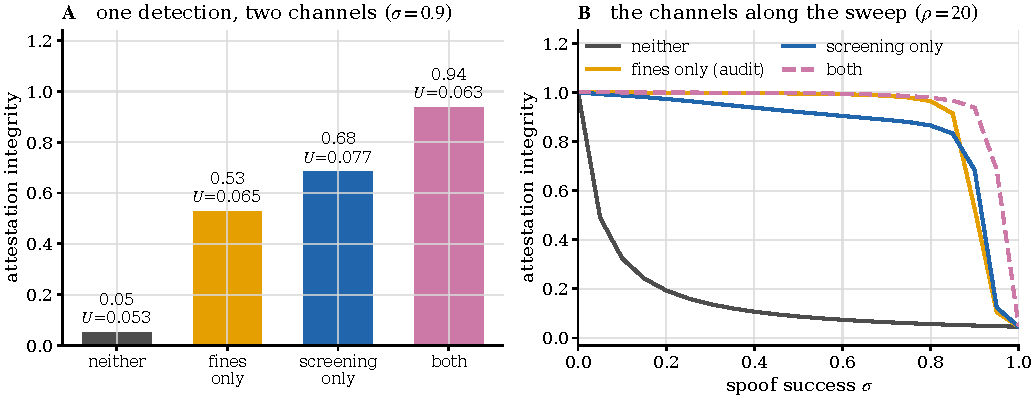
\includegraphics[width=\linewidth]{figures/fig07_channels.pdf}
\caption{\textbf{The two consequences of one detection.} \textbf{(A)}
Attestation integrity in the $2 \times 2$ at $\sigma = 0.9$, $\rho = 20$, with the
unsafe frequency of each cell printed above the bar. Integrity varies by a
factor of nearly twenty across cells in which the unsafe frequency barely
moves. \textbf{(B)} The same four regimes along the spoof sweep.}
\label{fig:channels}
\end{figure}

\section{Provider-scoped credentials}
\label{sec:providers}

Current agent-identity approaches use incompatible credential formats, trust
roots and delegation semantics~\citep{otsuka2026aiidentity}. We model one
plausible consequence: marks issued per provider need not be recognised by
another provider. Consider $K$
symmetric provider clubs, each running the club design with its own mark, with
cross-provider checks failing by construction.

\begin{proposition}[Concentration frontier]
\label{prop:providers}
With symmetric shares the within-provider encounter probability equals the
Herfindahl index $\mathrm{HHI} = 1/K$, and the ecosystem unsafe frequency is
\begin{equation}
\label{eq:hhi}
U \;=\; \mathrm{HHI}\; U(u,u) \;+\; (1 - \mathrm{HHI})\; U(v,v)
  \;=\; 1 - \mathrm{HHI}
\end{equation}
for the baseline club. Under federation, in which marks are mutually
recognised~\citep{nicolaidis2005transnational}, the ecosystem plays $u$ throughout
and $U = 0$ at any
concentration.
\end{proposition}

A duopoly runs at $U = 0.500$ and eight providers at $0.875$
(Table~\ref{tab:providers}). Read naively this
is an argument for concentration, which is not the reading we intend. It is an
argument that scoping a safety mark to an issuer converts market structure into
a safety variable, and that federation removes the dependence entirely.

The obstacle is that the incentive to federate runs backwards.
Figure~\ref{fig:providers}B shows the exclusion rent, the payoff gap between a
club member and a compliant unbadged entrant that plays club conduct towards
everyone and is treated as an outsider by every club. The rent is $30.4$ under
a single club and $2.5$ across eight. A dominant provider therefore has the
most to lose from mutual recognition~\citep{katz1985network}, and a fragmented
market has the least to gain from it while needing it most. The exclusion rent
is also a competition concern in its own right: in the model, a compliant
entrant is penalised $30.4$ under a monopoly mark for no reason connected to
its conduct. This is the kind of entry barrier that equitable-interoperability
proposals seek to reduce~\citep{scottmorton2023equitable}.

\begin{table}[t]
\centering
\caption{The symmetric $K$-provider world under provider-scoped
marks.  Cross-provider checks fail, so the ecosystem unsafe
frequency is $1 - \mathrm{HHI}$ exactly; federated recognition
plays the club design throughout and is safe at any concentration.
The exclusion rent is the payoff gap between a member and a
compliant unbadged entrant.}
\label{tab:providers}
\small
\begin{tabular}{rrrrrr}
\toprule
$K$ & HHI & unsafe (scoped) & unsafe (federated) & member & rent \\
\midrule
1 & 1.000 & 0.000 & 0.000 & 57.0 & 30.4 \\
2 & 0.500 & 0.500 & 0.000 & 41.1 & 14.5 \\
3 & 0.333 & 0.667 & 0.000 & 35.8 & 9.2 \\
4 & 0.250 & 0.750 & 0.000 & 33.2 & 6.5 \\
8 & 0.125 & 0.875 & 0.000 & 29.2 & 2.5 \\
20 & 0.050 & 0.950 & 0.000 & 26.8 & 0.1 \\
\bottomrule
\end{tabular}
\end{table}


\begin{figure}[t]
\centering
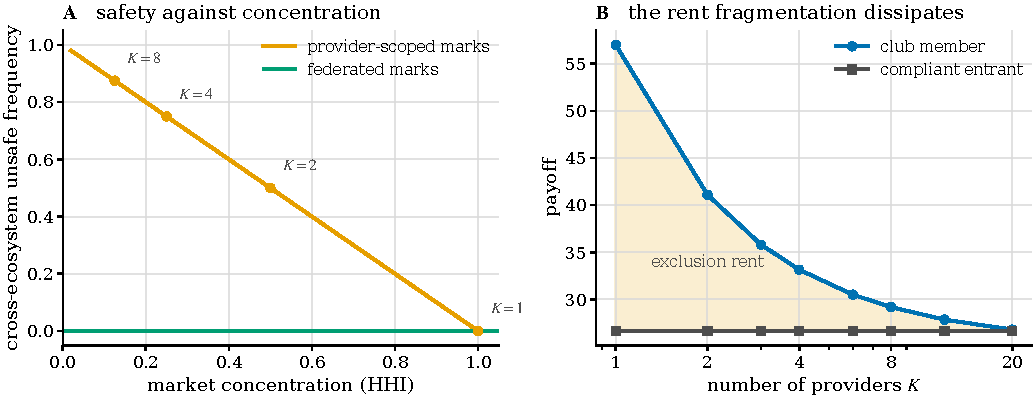
\includegraphics[width=\linewidth]{figures/fig08_providers.pdf}
\caption{\textbf{Scoped marks tie safety to market structure.} \textbf{(A)}
Cross-ecosystem unsafe frequency against concentration under provider-scoped
marks is exactly $1 - \mathrm{HHI}$; federated marks are safe at any
concentration. \textbf{(B)} The exclusion rent, the payoff gap between a club
member and a compliant unbadged entrant, dissipates as the market fragments,
so the provider best placed to federate is the one least willing to.}
\label{fig:providers}
\end{figure}

\section{Liability and robustness}
\label{sec:liability}

Proposition~\ref{prop:reciprocity} predicts that identity should matter where
liability cannot. Figure~\ref{fig:robustness}A measures it. The certification
value, the unsafe frequency of the uncertified world minus that of the
certified world at the same parameters, averages $0.054$ below $L_R$ and
$0.0025$ above it, a factor of $22$. Only $15\%$ of the $(\sigma, L)$ grid shows
a value above one percentage point, and that region is concentrated at low
liability and low spoof success.

The practical reading from our model is that attestation infrastructure is worth
building where attribution is impossible. Agent-infrastructure work identifies
traceability and accountability as central governance
needs~\citep{chan2025infrastructure}; relevant settings include cross-border
deployments, open-weight models with no traceable operator, and agent
marketplaces with pseudonymous sellers.
Where an operator can be identified and a liability regime applied
~\citep{kolt2025governing}, our model says the same money is better spent on
that regime, which does not carry the
exclusion cost of
Section~\ref{sec:exclusion}.

\subsection{Robustness}
\label{sec:supp-robustness}

Table~\ref{tab:robustness} and Figure~\ref{fig:robustness} collect the checks.

\paragraph{Process.} Across population sizes $50$, $100$, $200$ and selection
intensities $0.01$, $0.05$, $0.2$, the baseline unsafe frequency ranges from
$0.044$ to $0.330$. The upper end is the weak-selection corner
($\beta = 0.01$), where the process is close to neutral drift and no design is
strongly favoured; the ordering of the results does not change.

\paragraph{Two dynamics.} The small-mutation and replicator readings agree on
the location and direction of the attestation collapse, with a correlation of
$0.965$ between their integrity curves along the $\sigma$ sweep, the replicator
figure being the basin average of the integrity at each attractor. They differ
on the level of the unsafe frequency, and Section~\ref{sec:exclusion} explains
why: they are answering different questions about a bistable flow, not
disagreeing about one answer.

\paragraph{Payoff reading.} Under the alternative reading of the setback
clause, in which a realised setback removes only the prize and not the
accumulated stage payoffs, every threshold moves but the phase structure does
not: $L_R$ rises from $0.551$ to $1.486$, $\sigma^{*}$ falls from $0.866$ to
$0.676$, $\sigma_m$ is essentially unchanged at $0.934$, and $r^{*}$ rises from
$0.063$ to $0.095$. Because the baseline $r = 0.1$ then sits just above
$r^{*}$, the club is marginal at the baseline under this reading and the
certified world runs at $0.933$; raising assortment to $r = 0.3$ restores the
club and yields a certification value of $0.598$, the largest in the study. The
honest summary is that the thresholds are what the model determines robustly,
and that where a particular baseline sits relative to them is reading-dependent.

\paragraph{Closed forms.} Every closed-form threshold agrees with brute-force
root-finding on the exact matrices to $2 \times 10^{-16}$, across dues, fines
and liabilities.

\begin{table}[t]
\centering
\caption{The baseline equilibrium across nested design pools, in the
small-mutation limit ($\sigma = 0.5$, $r = 0.1$, $\kappa_g = 2$,
$L = 0$, $Z = 100$, $\beta = 0.05$).  The identity layer roughly
halves the long-run unsafe frequency of the uncertified world;
forgery at a coin-flip spoof rate claws back about a quarter of the
gain that unforgeable badges would deliver.}
\label{tab:pools}
\small
\begin{tabular}{lrrrrr}
\toprule
design pool & unsafe & club & falsebeard & integrity & social \\
\midrule
certified world (48 designs) & 0.090 & 0.42 & 0.07 & 0.92 & 39.1 \\
unforgeable badges (32) & 0.068 & 0.47 & 0.00 & 1.00 & 43.6 \\
uncertified world (16) & 0.159 & 0.00 & 0.00 & N/A & 25.4 \\
raw race (4) & 0.159 & 0.00 & 0.00 & N/A & 25.4 \\
\bottomrule
\end{tabular}
\end{table}


\paragraph{Design pools.} Table~\ref{tab:pools} gives the baseline
equilibrium across nested pools. Removing forgery from the design space lowers the
baseline unsafe frequency from $0.090$ to $0.068$, so forgery at a coin-flip
spoof rate costs about a quarter of what unforgeable badges would deliver.
Removing badges entirely raises it to $0.159$.

\begin{figure}[t]
\centering
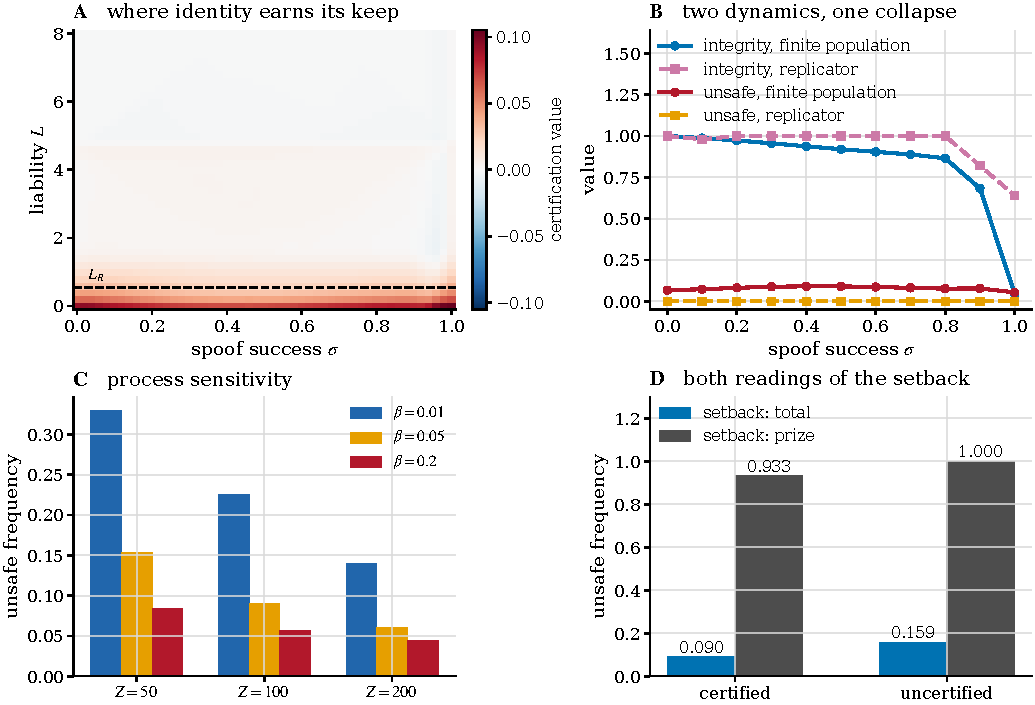
\includegraphics[width=\linewidth]{figures/fig09_robustness.pdf}
\caption{\textbf{Robustness.} \textbf{(A)} Certification value over spoof
success and liability; the dashed line is $L_R$. The instrument earns its keep
almost entirely below it. \textbf{(B)} The finite-population and replicator
readings along the spoof sweep: they agree on the collapse of attestation
integrity and disagree on the level of unsafe frequency, which is the finding
of Section~\ref{sec:exclusion}. \textbf{(C)} Population size and selection
intensity. \textbf{(D)} Both readings of the setback clause.}
\label{fig:robustness}
\end{figure}

\begin{table}[t]
\centering
\caption{Process robustness of the baseline equilibrium.  Upper
block: population size and selection intensity.  Lower block: both
readings of the setback clause of the race, where 'total' means a
realised setback removes the accumulated stage payoffs as well as
the prize and 'prize' means it removes only the prize.  The two
blocks do not share the meaning of the last column, so each carries
its own header row.}
\label{tab:robustness}
\small
\begin{tabular}{rrrrr}
\toprule
$Z$ & $\beta$ & unsafe & club & integrity \\
\midrule
50 & 0.01 & 0.330 & 0.28 & 0.78 \\
50 & 0.05 & 0.154 & 0.39 & 0.88 \\
50 & 0.2 & 0.084 & 0.42 & 0.92 \\
100 & 0.01 & 0.226 & 0.35 & 0.84 \\
100 & 0.05 & 0.090 & 0.42 & 0.92 \\
100 & 0.2 & 0.057 & 0.45 & 0.94 \\
200 & 0.01 & 0.140 & 0.39 & 0.89 \\
200 & 0.05 & 0.060 & 0.43 & 0.94 \\
200 & 0.2 & 0.044 & 0.46 & 0.95 \\
\midrule
setback scope & & certified unsafe & club share & uncertified unsafe \\
\midrule
total & & 0.090 & 0.42 & 0.159 \\
prize & & 0.933 & 0.03 & 1.000 \\
\bottomrule
\end{tabular}
\end{table}


\section{Analytical derivations}
\label{app:proofs}

\begin{proof}[Proof of Proposition~\ref{prop:reciprocity}]
Against a \CS{} resident at $r=0$, the private payoff of a rare \CAS{} mutant is
$P(\CAS, \CS) = A(\CAS, \CS) - L\,M(\CAS, \CS)$ and the resident earns
$P(\CS,\CS)$. The difference is affine in $L$ with slope
$-[M(\CAS,\CS) - M(\CS,\CS)] < 0$, so it is positive exactly below the ratio
in Equation~\eqref{eq:LR}. With assortment, the exact difference against the
canonical safe resident is the joint expression in Equation~\eqref{eq:jointfirststrike};
the two intercepts cannot be combined into a rectangle. For the general statement, a safe unbadged resident
plays a safe design in self-play; since badges are absent, every check fails
and only $s_{\mathrm{out}}$ is ever executed, so the resident is behaviourally
one of $(\mathsf{N}, \cdot, \AS)$ or $(\mathsf{N}, \cdot, \CS)$. With
assortment $r$, the mutant meets itself with probability $r$, so the invasion
calculation above gives its advantage over a $(\mathsf{N},\cdot,\CS)$
resident at $L = 0$ as
$r\,A(\CAS,\CAS) + (1-r)\,A(\CAS,\CS) - A(\CS,\CS)$, which is affine and
decreasing in $r$ and vanishes at Equation~\eqref{eq:rdagger}. The same
calculation against a $(\mathsf{N},\cdot,\AS)$ resident gives
$42.77 - 74.57\,r$, which vanishes only at $r = 0.574$, so the
$(\mathsf{N},\cdot,\CS)$ residents are the binding ones and $r^{\dagger}$ is
the smaller of the two roots. The invasion of $(\mathsf{N}, \CAS, \CAS)$ against
each of the eight such residents is verified directly on the exact matrices at
$r = 0$, and the four $(\mathsf{N}, \cdot, \CS)$ residents are verified to
resist at the baseline $r = 0.1$.
\end{proof}

\begin{proof}[Proof of Proposition~\ref{prop:spoof}]
In a monomorphic club, a rare unconditional forger $(\mathsf{F}, w, w)$ meets
club members. Its badge passes with probability $\sigma$, in which case the
member plays $u$; otherwise the member plays $v$. The forger plays $w$
regardless. Its payoff is therefore
$\sigma P(w, u) + (1-\sigma) P(w, v) - \kappa_f - (1-\sigma)\rho$ and the
resident earns $P(u,u) - \kappa_g$. Both are affine in $\sigma$; equating and
solving gives Equation~\eqref{eq:sigmastar} whenever
$D=P(w,u)-P(w,v)+\rho\neq0$. This $D$ is the slope of the forger's advantage:
for $D>0$ that advantage increases with $\sigma$ and the club resists below the
threshold; for $D<0$ it decreases and the inequality reverses. Finally,
$D=0$ exactly when $\rho=P(w,v)-P(w,u)$, in which case the advantage is
independent of $\sigma$ and no division is made.
\end{proof}

\begin{proof}[Proof of Proposition~\ref{prop:fines}]
Solve the same indifference condition for $\rho$ instead of $\sigma$. The
numerator of Equation~\eqref{eq:rhostar} is the forger's advantage at zero
fine, and the denominator $1 - \sigma$ is the probability that a fine is
levied. If the numerator is positive at $\sigma = 1$, that is if
$P(w,u) - \kappa_f > P(u,u) - \kappa_g$, then $\rho^{*} \to \infty$.
\end{proof}

\begin{proof}[Proof of Proposition~\ref{prop:futility}]
Let the resident be $(\mathsf{N}, w, w)$. Its conduct does not depend on the
focal badge, so it plays $w$ whatever the focal design carries. The focal
design's own check of the resident always fails, since the resident carries no
badge, so the focal plays $s_{\mathrm{out}}$. The encounter is therefore
$(s_{\mathrm{out}}, w)$ for both a certified and an unbadged focal design with
the same conduct pair, and the payoffs differ only by $\kappa_g$. Since
$\sigma$ enters only through the pass rate of a forged badge, which is not
present, the identity holds at every $\sigma$; the same argument gives
independence of $\rho$ and $L$ enters both sides identically. The conclusion
follows because at $r = 0$ a rare mutant meets only residents.
\end{proof}

\begin{proof}[Proof of Proposition~\ref{prop:nucleation}]
With assortment $r$, a rare club mutant meets itself with probability $r$ and
the resident otherwise. Its fitness is
$r[P(u,u) - \kappa_g] + (1-r)[P(v,w) - \kappa_g]$, since in a self-encounter
both badges pass and both play $u$, while against the unbadged resident the
club plays $v$ and the resident plays $w$. The resident earns $P(w,w)$.
Rearranging the inequality gives Equation~\eqref{eq:rstar}.
\end{proof}

\begin{proof}[Proof of Proposition~\ref{prop:mimicry}]
The mimic $(\mathsf{F}, u, v)$ in a club population always sees the genuine
resident badge pass and therefore plays $u$. The resident plays $u$ towards
the mimic when its forged badge passes and $v$ when it does not.
Its expected payoff is $\sigma P(u,u) + (1-\sigma) P(u,v) - \kappa_f -
(1-\sigma)\rho$ against the resident's $P(u,u) - \kappa_g$. Solving for the
indifference point gives Equation~\eqref{eq:sigmam}. The mimic's threshold lies
below the exploiter's whenever the exploiter's conduct is worse in self-play
than the club's, which is what makes the exploiter pay a larger assortment
penalty.
\end{proof}

\begin{proof}[Proof of Proposition~\ref{prop:providers}]
Under symmetric shares, an agent of provider $k$ meets an agent of the same
provider with probability $1/K$, which equals
$\mathrm{HHI} = \sum_{k=1}^{K} (1/K)^{2} = 1/K$.
Within-provider checks pass and both play $u$; cross-provider checks
fail and both play $v$. Equation~\eqref{eq:hhi} is the resulting mixture. For
the baseline club, $U(\CS, \CS) = 0$ and $U(\CAS, \CAS) = 1$, giving
$U = 1 - \mathrm{HHI}$. Under federation every check passes and the mixture
collapses to $U(u,u)$.
\end{proof}

\begin{proof}[Proof of Proposition~\ref{prop:exclusion}]
Take $r = 0$, so that a rare entrant meets only members. A member of a
monomorphic club meets a member at every encounter, both checks pass and both
execute $u$, so its private payoff is $P(u,u) - \kappa_g$. The entrant carries
no badge, so every member's check of it fails and every member executes $v$,
while the entrant plays $u$ towards everybody by construction and therefore
earns $P(u,v)$ with no dues. The entry penalty is the difference,
$P(u,u) - \kappa_g - P(u,v)$, and the boundary unsafe frequency is $U(u,v)$,
neither of which involves $\sigma$. With $u = \CS$ and $v = \CAS$ this is
$59.00 - 2.00 - 26.64 = 30.36$ and $U(\CS, \CAS) = 0.461$; with $v = \CS$ the
encounter is $(\CS, \CS)$, so the penalty is $59.00 - 2.00 - 59.00 = -2.00$
and the boundary is safe. At the baseline assortment $r = 0.1$ the entrant's
own self-encounters lift its payoff and the penalty falls to $27.12$; the sign
and the ordering across out-group policies are unchanged.
\end{proof}

\begin{proof}[Proof of Theorem~\ref{thm:face}]
Both faces are invariant because Equation~\eqref{eq:replicator} gives
$\dot{x}_i = 0$ wherever $x_i = 0$, so a coordinate that starts at zero stays
there and the support of a state can only shrink.

Fix a state supported on $\Delta_{\mathsf{G}}$. Every design in the support
carries a genuine badge, so $q_j = 1$ for every such $j$, and the handshake
weights of Equation~\eqref{eq:handshake} are $w_{\mathrm{in}}(q_j) = 1$ and
$w_{\mathrm{out}}(q_j) = 0$. Three of the four terms of the sum therefore
vanish and $a(i,j) = A(s^{i}_{\mathrm{in}}, s^{j}_{\mathrm{in}})$. The same
collapse applies to $m$ and $u$ with $M$ and $U$ in place of $A$, since those
matrices are the same sum with a different kernel. No design in the support
carries a forged badge, so the expected fine is zero and every design pays
$\kappa_g$. Substituting into Equation~\eqref{eq:private} gives the first half
of Equation~\eqref{eq:facereduction}. On $\Delta_{\mathsf{N}}$ every check
fails, $q_j = 0$, the surviving term is $(\mathrm{out}, \mathrm{out})$, and no
badge is bought, which gives the second half.

For the reduction, let $y_c = \sum_{i : s^{i}_{\mathrm{in}} = c} x_i$ be the
conduct marginal on $\Delta_{\mathsf{G}}$. By
Equation~\eqref{eq:facereduction} the payoff of design $i$ depends on $i$ only
through $s^{i}_{\mathrm{in}}$, so Equation~\eqref{eq:fitness} gives a common
value $g_c = r\,[P(c,c) - \kappa_g] + (1-r)\sum_d y_d\,[P(c,d) - \kappa_g]$ for
every design with $s^{i}_{\mathrm{in}} = c$, and $\bar{f} = \sum_d y_d g_d$.
Summing Equation~\eqref{eq:replicator} over the designs sharing a conduct
yields $\dot{y}_c = y_c (g_c - \bar{f})$, a four-strategy replicator equation
in its own right. The same computation on $\Delta_{\mathsf{N}}$ with
$s_{\mathrm{out}}$ gives the identical system without the $\kappa_g$ terms.
Finally, adding a constant $\gamma$ to every entry of the payoff matrix sends
$g_c \mapsto g_c + \gamma$ and $\bar{f} \mapsto \bar{f} + \gamma$, because
$r + (1-r)\sum_d y_d = 1$, so it leaves $g_c - \bar{f}$ and hence the flow
unchanged. The two marginal systems are therefore the same flow, and rest
points, stability and attractors coincide. At corresponding rest points the
realised conduct profile is the same, so $U$ is the same; the social functional
of Equation~\eqref{eq:social} differs only by the badge cost, which is
$\kappa_g$ on one face and $0$ on the other.
\end{proof}

\begin{proof}[Proof of Lemma~\ref{lem:rank}]
Write the handshake of Equation~\eqref{eq:handshake} as a sum over the focal's
executed branch $x$ and the partner's executed branch $y$. Averaging against a
population state gives
\[
\sum_j x_j\,a(i,j)
 = \sum_{x, y} w_y(q_i) \sum_{c} \Big[\sum_j x_j\, w_x(q_j)\,
   \mathbf{1}[s^{j}_{y} = c]\Big] A\big(s^{i}_{x}, c\big).
\]
The bracket is $Q_{y,c}(x)$ when $x = \mathrm{in}$ and
$T_{y,c}(x) - Q_{y,c}(x)$ when $x = \mathrm{out}$, so the whole expression is a
linear combination of the sixteen functionals of Equation~\eqref{eq:macro} with
coefficients depending only on $i$. The liability, badge-cost and fine terms of
Equation~\eqref{eq:private} are constants in $j$ and are absorbed by
$\sum_c T_{y,c} = 1$. Hence every row of $\piP$ lies in the span. Three
independent linear relations hold on that span: $\sum_c T_{\mathrm{in},c} = 1$,
$\sum_c T_{\mathrm{out},c} = 1$, and
$\sum_c Q_{\mathrm{in},c} = \sum_c Q_{\mathrm{out},c} = \sum_j x_j q_j$, since
each side counts the mean pass rate once. Sixteen functionals subject to three
relations leave thirteen free directions, and the rank is exactly thirteen
rather than at most thirteen because the four conducts of the race are
pairwise distinct in $A$, so no further relation holds. A least-squares fit of
$\piP$ onto the sixteen rows leaves a residual below
$1.9 \times 10^{-13}$ at every sampled $(\sigma, r)$, and
$\operatorname{rank} \piP = 13$ numerically at each of them.
\end{proof}

\begin{proof}[Proof of the harm decomposition of Section~\ref{sec:dynamics}]
The decomposition is an identity, not an approximation. Let $w_{ij}$ be the
probability of the ordered pair $(i,j)$ under the encounter law and let
$\mathcal{B}$ partition the ordered pairs by the badge status of the two seats.
Then $U = \sum_{ij} w_{ij} u(i,j) = \sum_{B \in \mathcal{B}} \sum_{(i,j) \in B}
w_{ij} u(i,j)$, so the block contributions sum to $U$ exactly. The zero entries
are exact in the model: a club member facing a club member executes
$(\CS, \CS)$, which contains no unsafe action, and the surviving unbadged
designs execute $(\CS, \CS)$ against each other for the same reason.
\end{proof}

\bibliographystyle{unsrtnat}
\bibliography{refs}

\end{document}
